\section{Variational Autoencoders}
\label{sec:vae}
Variational Autoencoders (VAE) have been developed concurrently in 2014 by Kingma and Welling \cite{vae:2014} and Rezende et al\cite{dlgm:2014}.
VAEs couple a generator network with an inference network in which efficient inference and learning can be performed, thus allowing the model to be trained purely using gradient-based methods.

%which uses variational inference to perform efficient inference and learning in deep latent models.
%Deep latent models are based on the assumption that input data can be explained using non-linear transformations coming from simple distributions. \cite{rezende:2014} (check!?).

\paragraph{Variational Inference (VI)} is a method for approximating intractable posterior distributions over a set of hidden varibales given observations.
More specifically, VI turns the inference problem of computing $p(z|x)$ where $z$ are hidden and $x$ observed variables into an optimization problem.
The term \emph{variational} derives from the calculus of variations, which is a field in mathematical analysis dealing with choosing the best function $q$ from a set of functions $Q$. In the case of variational inference, this $Q$ denotes a class of distributions and the variational parameters are the parameters which are used to define $q \in Q$.
VI is a alternative to markov chain monte carlo (MCMC) methods like gibbs sampling, due to lower computational cost.
However, there is no guarantee that VI methods will asymptotically reach the optimimum in contrast to MCMC.

Given this assumption, building a good representation in the latent space is crucial for minimal reconstruction error as well as good generative modelling in practice(?).

% TODO: add clarification that q/p are deep nets!
\begin{figure}[htb]
\centering
\includestandalone[width=\linewidth,mode=buildnew]{media/vae_conceptual}
  \caption{VAE architecture (source: VAE paper)}\label{fig:vae_architecture}
\end{figure}

\newpage

\paragraph{Formal Setup}
Formally, $p(x,z)$ is the joint probability distribution over both input and latent variables while $p(z|x)$ is the conditional probability of the latent variables given input data.
Inferring the posterior distribution $p(z|x)$ is particularly interesting, because it means to enable learning parameters for good latent space representation.
$p(z|x)$ can be expanded using bayes rule to $\frac{p(x|z) p(z)}{p(x)}$.
Computing the nominator is straightforward, $p(z)$ is the probability distribution we chose for the latent space, oftenmost simply a gaussian.
$p(x|z)$ is easy to compute as well, ...? (forward pass?).\\
Meanwhile is the denominator difficult to evaluate, because it requires to consider all possible input combinations.
What we do instead in the variational autoencoders is to derive a lower-bound on $p(z|x)$ using a auxiliary distribution called $q_\theta(z|x)$. The subscript $\theta$ indicates that the distribution is parametrized by an variational term, so that for one $\theta$, $q_\theta(z|x) \approxeq p(z|x)$ holds ($q(z|x)$ doesn't need to depend on $x$).
%Performing statistical inference means computing $p(z|x)$ which is intractable in all but very simple cases (integrating over it, show calc).

%In this setup we have observed variables $x$ from which we would like to infer latent variables $z$


%Variational Autoencoders (VAE) have been a popular choice for unsupervised learning of complicated distributions (citation needed) and generative modelling.
%In order to generate data from unknown and mostly intractable distributions, we need approximations.
%There are basically two approaches for sampling from these distributions,
%first there are approximate samples (MCMC, gibbs sampling, etc) which try to directly approximate $p(x)$.
%Variational Autoencoders instead try to match an easier to compute distribution $q(x)$ to $p(x)$.
%By using this approach, VAEs are computationally less intensive (citation?) but have the drawback of being more restricted in their modelling approach.
%Practically, this means that with more computation MCMC methods approach $p(x)$, while there is no such guarantee for variational methods (--> not for all).

%VAE can be learned with just backpropagation (paper,TODO), but they differ from denoising and sparse autoencoders due to the different loss function.


%VAEs are built on top of neural networks and are designed in a way to allow training with gradient-based methods.
%Learning and inference are reasonable efficient and relatively easy to implement and show decent results, but have been overshadowed by more recent adversarial approaches (citation needed!!,see \ref{sec:gan}).

\subsection{Architecture}
\label{sub:vae_architecture}

\begin{figure}[htb]
\centering
\resizebox{5cm}{!}{\definecolor{cdfdfdf}{RGB}{223,223,223}
\definecolor{cffffff}{RGB}{255,255,255}


\begin{tikzpicture}[y=0.80pt, x=0.80pt, yscale=-1.000000, xscale=1.000000, inner sep=0pt, outer sep=0pt]
\begin{scope}[cm={{1.25,0.0,0.0,-1.25,(0.0,1052.3622)}}]
  \begin{scope}[shift={(306.491,697.587)}]
    \path[draw=black,fill=cdfdfdf,line join=miter,line cap=butt,miter
      limit=10.00,nonzero rule,line width=0.319pt] (9.9628,0.0000) .. controls
      (9.9628,5.5023) and (5.5023,9.9628) .. (0.0000,9.9628) .. controls
      (-5.5023,9.9628) and (-9.9628,5.5023) .. (-9.9628,0.0000) .. controls
      (-9.9628,-5.5023) and (-5.5024,-9.9628) .. (0.0000,-9.9628) .. controls
      (5.5023,-9.9628) and (9.9628,-5.5024) .. (9.9628,0.0000) -- cycle;
  \end{scope}
    \path[cm={{1.0,0.0,0.0,-1.0,(303.468,695.373)}},fill=black,nonzero rule]
      (0.0000,0.0000) node[above right] (text4171) {$x$};
  \begin{scope}[shift={(306.491,697.587)}]
    \path[draw=black,fill=cffffff,line join=miter,line cap=butt,miter
      limit=10.00,nonzero rule,line width=0.319pt] (9.9628,48.6708) .. controls
      (9.9628,54.1732) and (5.5024,58.6336) .. (0.0000,58.6336) .. controls
      (-5.5023,58.6336) and (-9.9628,54.1732) .. (-9.9628,48.6708) .. controls
      (-9.9628,43.1685) and (-5.5024,38.7081) .. (0.0000,38.7081) .. controls
      (5.5023,38.7081) and (9.9628,43.1685) .. (9.9628,48.6708) -- cycle;
  \end{scope}
    \path[cm={{1.0,0.0,0.0,-1.0,(303.945,744.043)}},fill=black,nonzero rule]
      (0.0000,0.0000) node[above right] (text4181) {$z$};
    \path[cm={{1.0,0.0,0.0,-1.0,(260.848,741.767)}},fill=black,nonzero rule]
      (0.0000,0.0000) node[above right] (text4187) {$\phi$};
    \path[cm={{1.0,0.0,0.0,-1.0,(345.199,742.798)}},fill=black,nonzero rule]
      (0.0000,0.0000) node[above right] (text4193) {$\theta$};
  \begin{scope}[shift={(306.491,697.587)}]
    \path[draw=black,dash pattern=on 2.39pt off 2.39pt,line join=miter,line
      cap=butt,miter limit=10.00,line width=0.319pt] (-38.5088,48.6708) --
      (-10.9710,48.6708);
  \end{scope}
  \begin{scope}[shift={(295.52,746.258)}]
    \path[draw=black,fill=black,line join=miter,line cap=butt,miter
      limit=10.00,nonzero rule,line width=0.319pt] (-5.2035,2.3356) --
      (0.2989,0.0000) -- (-5.2035,-2.3356) -- (-5.2035,2.3356) -- cycle;
  \end{scope}
  \begin{scope}[shift={(306.491,697.587)}]
    \path[draw=black,line join=miter,line cap=butt,miter limit=10.00,line
      width=0.319pt] (38.5088,48.6708) -- (10.9710,48.6708);
  \end{scope}
  \begin{scope}[cm={{-1.0,0.0,0.0,-1.0,(317.462,746.258)}}]
    \path[draw=black,fill=black,line join=miter,line cap=butt,miter
      limit=10.00,nonzero rule,line width=0.319pt] (-5.2035,2.3356) --
      (0.2989,0.0000) -- (-5.2035,-2.3356) -- (-5.2035,2.3356) -- cycle;
  \end{scope}
  \begin{scope}[shift={(306.491,697.587)}]
    \path[draw=black,line join=miter,line cap=butt,miter limit=10.00,line
      width=0.319pt] (38.5088,45.5084) -- (7.1087,8.4005);
  \end{scope}
  \begin{scope}[cm={{-0.64792,-0.7657,0.7657,-0.64792,(313.6,705.988)}}]
    \path[draw=black,fill=black,line join=miter,line cap=butt,miter
      limit=10.00,nonzero rule,line width=0.319pt] (-5.2035,2.3356) --
      (0.2989,0.0000) -- (-5.2035,-2.3356) -- (-5.2035,2.3356) -- cycle;
  \end{scope}
  \begin{scope}[shift={(306.491,697.587)}]
    \path[draw=black,dash pattern=on 2.39pt off 2.39pt,line join=miter,line
      cap=butt,miter limit=10.00,line width=0.319pt] (-7.1856,7.1856) .. controls
      (-16.6444,16.6438) and (-16.6444,32.0271) .. (-7.7582,40.9132);
  \end{scope}
  \begin{scope}[cm={{0.7071,0.7071,-0.7071,0.7071,(298.733,738.5)}}]
    \path[draw=black,fill=black,line join=miter,line cap=butt,miter
      limit=10.00,nonzero rule,line width=0.319pt] (-5.2035,2.3356) --
      (0.2989,0.0000) -- (-5.2035,-2.3356) -- (-5.2035,2.3356) -- cycle;
  \end{scope}
  \begin{scope}[shift={(306.491,697.587)}]
    \path[draw=black,line join=miter,line cap=butt,miter limit=10.00,line
      width=0.319pt] (0.0000,38.5088) -- (0.0000,10.9710);
  \end{scope}
  \begin{scope}[cm={{0.0,-1.0,1.0,0.0,(306.491,708.558)}}]
    \path[draw=black,fill=black,line join=miter,line cap=butt,miter
      limit=10.00,nonzero rule,line width=0.319pt] (-5.2035,2.3356) --
      (0.2989,0.0000) -- (-5.2035,-2.3356) -- (-5.2035,2.3356) -- cycle;
  \end{scope}
    \path[cm={{1.0,0.0,0.0,-1.0,(308.318,675.918)}},fill=black,nonzero rule]
      (0.0000,0.0000) node[above right] (text4239) {N};
  \begin{scope}[shift={(306.491,697.587)}]
    \path[draw=black,line join=miter,line cap=butt,miter limit=10.00,line
      width=0.319pt] (16.5376,62.3527) -- (-16.5376,62.3527) .. controls
      (-18.7386,62.3527) and (-20.5228,60.5685) .. (-20.5228,58.3676) --
      (-20.5228,-21.2037) .. controls (-20.5228,-23.4046) and (-18.7386,-25.1888) ..
      (-16.5376,-25.1888) -- (16.5376,-25.1888) .. controls (18.7386,-25.1888) and
      (20.5228,-23.4046) .. (20.5228,-21.2037) -- (20.5228,58.3676) .. controls
      (20.5228,60.5685) and (18.7386,62.3527) .. (16.5376,62.3527) -- cycle;
  \end{scope}
\end{scope}

\end{tikzpicture}

}
  \caption{VAE architecture (source: VAE paper)}\label{fig:vae_architecture}
\end{figure}
VAE just like other autoencoders encode the input data into a latent space similar to compression of data and is able to decode a vector of latent variables into output while trying to match the output to the input.
But in contrast to other autoencoders (sparse, denoising), we enforce a specific distribution on the latent space.
This allows to sample from this distribution and generate output which will look similar to the data on which the VAE has been trained.
\ref{fig:vae_architecture}.

\paragraph{Relation to Auto-Encoders}
The variational autoencoder has the same encoding-decoding architecture as other autoencoders, for example sparse or denoising autoencoders.
But in contrast to these autoencoders, the VAE enforces a probability distribution on the learned latent space $z$.
In particular, the framework encourages the model to learn a representation that is close to $p(z)$ (which usually is an isotropic multivariate gaussian distribution) by including the KL divergence in the objective function.
%Similar to other autoencoder frameworks VAE provides an encoder as well as a decoder model, but in contrast to other autoencoders both networks are probabilistic. This means that the model described by the VAE framework can be seen as a jointly trained probabilistic encoder and probabilistic decoder.
%One of the main differences is that the VAE framework enforces a specific prior distribution on the latent space, most of the time simply an isotropic gaussian.



\paragraph{The Kullback-Leibler Divergence} (KL divergence) is a measurement for the difference between two probability distributions. $\mathcal{D}_{\mathrm{KL}}(P \| Q)$ can informally described as the amount of information which is lost when using $Q$ to represent $P$.
The KL divergence does not obey the triangle inequality and is also not symmetrical, therefore it does not qualify as a metric.
$\mathcal{D}_{\mathrm{KL}}(P||Q)$ can nevertheless be understood as a measure of the difference between $P$ and $Q$ and is as such used in the VAE to approximate the true posterior distribution.

\subsection{Objective Function}
The objective function of the VAE consists of the reconstruction error and the regularizer.
%$\mathcal{L}$ learns both the encoder as well as the decoder with their respective parameters $\phi$ and $\theta$.
% probabilistic encoder $q_\phi(z|x)$ (produces z values from which x could've been generated)
% probabilistic decoder $p_\theta(x|z)$
We will discuss both terms in detail below following the derivation of the lower variational bound $\mathcal{L}$ and the rewritten objective function.

\paragraph{Derivation of lower bound}
Based on \cite[p.~698]{deeplearning:2016}.
\begin{align*}
  \log p(x)\\
  &= \int_z q_\phi(z|x) \log p(x) dz\\
  &= \int_z q_\phi(z|x) \log \frac{p_\theta(x,z)}{p_\theta(z|x)} dz \tag{Bayes' rule}\\
  &= \int_z q_\phi(z|x) \log\bigg(\frac{p_\theta(z,x)}{q_\phi(z|x)} \frac{q_\phi(z|x)}{p_\theta(z|x)}\bigg) dz \tag{Chain rule}\\
  &= \int_z q_\phi(z|x) \bigg(\log\frac{p_\theta(z,x)}{q_\phi(z|x)} + \log\frac{q_\phi(z|x)}{p_\theta(z|x)}\bigg) dz\\
  &= \int_z q_\phi(z|x) \log \frac{p_\theta(z,x)}{q_\phi(z|x)} dz + \int_z q_\phi(z|x) \log\frac{q_\phi(z|x)}{p_\theta(z|x)} dz\\
  &= \underbrace{\int_z q_\phi(z|x) \log \frac{p_\theta(z,x)}{q_\phi(z|x)} dz}_{= \mathcal{L}}+ \underbrace{\mathcal{D}_{\mathrm{KL}}\big(q_\phi(z|x) \| p_\theta(z|x)\big) dz}_{\geq 0}\\
  &\geq \mathcal{L}\\
\end{align*}

$\mathcal{L}$ is called the evidence lower bound with respect to $\log p(x)$.
We further rewrite $\mathcal{L}$ in order decompose the term into two separate terms, the reconstruction error $\mathcal{L}_{rec}$ and the regularizer $\mathcal{L}_{reg}$.

\begin{align*}
  \mathcal{L}
  &= \int q_\phi(z|x) \log\frac{p_\theta(z,x)}{q_\phi(z|x)} dz\\
  &= \int q_\phi(z|x) \log\frac{p(z) p_\theta(x|z)}{q_\phi(z|x)} \tag{we assume that x is conditionally dependent on z} dz\\
  &= \int q_\phi(z|x) \bigg(\log\frac{p(z)}{q_\phi(z|x)} + \log p_\theta(x|z)\bigg) dz\\
  &= -\int q_\phi(z|x) \log\frac{q_\phi(z|x)}{p(z)} dz + \int q_\phi(z|x) \log p_\theta(x|z) dz\\
  &= -\mathcal{D}_{\mathrm{KL}}\big(q_\phi(z|x) \| p(z)\big) + \int q_\phi(z|x) \log p_\theta(x|z) dz\\
  &= \underbrace{-\mathcal{D}_{\mathrm{KL}}\big(q_\phi(z|x) \| p(z)\big)}_{\mathcal{L}_{reg}} + \underbrace{\mathbb{E}_{z \sim q_\phi(z|x)}\big[ \log p_\theta(x|z)\big]}_{\mathcal{L}_{rec}}\\
  &= \mathcal{L}_{reg} + \mathcal{L}_{rec}
\end{align*}


\paragraph{Regularization term $\mathcal{L}_{reg}$} encourages the model to learn simple representations in latent space, due to the negative Kullback-Leibler (KL) divergence between the learned variational distribution $q_\theta(z|x)$ and the latent space prior distribution $p(z)$.
The regularizer also prevents the model from collapsing into a single point.

\vspace{10cm}
% move to architecture:
%In the original VAE paper, the unit gaussian distribution with diagonal variance was proposed for $p(z)$ and although there have been multiple proposals (citations, multi-modal etc) for different distributions we will stick with $\mathcal{N}(0,I)$ for the sake of simplicity.
% ---

%For two probability distributions $P$ and $Q$, the KL divergence $\mathcal{D}_{\mathrm{KL}}(P||Q)$ can informally be described as the amount of information which is lost when using $Q$ to represent $P$.

\paragraph{Reconstruction error $\mathcal{L}_{rec}$} measures how well the decoder reconstructs the input data using the latent space $z$.
This error is measures using the negative log-likelihood of the conditional probability distribution $p_\theta(x_i|z)$ where $z$ is sampled from $q_\phi(z | x_i)$.
$\mathcal{L}_{\mathrm{rec}}$ is necessary to force the encoder to produce latent variables which can be used to reconstruct the input data well.


%\begin{figure}[htb]
%\centering
%\includestandalone[width=\linewidth,mode=buildnew]{media/vae_multiple_layers}
  %\caption{VAE with multiple stochastic layers }\label{fig:vae_multiple_layers}
  %\medskip
  %\small
  %The left upward arrows indicate the recognition networks $q(h_1|x)$ and $q(h_2|h_1)$.
  %Note that the recognition networks can have multiple deterministic layers (including non-linearities).\\

  %$p(h_2)$ denotes the probability distribution over the highest(?) latent space.\\

  %On the right, the two conditional distributions $p(h_1|h_2)$ and $p(x|h_2)$ are representing two networks used for the generative process.
%\end{figure}


\newpage

\subsubsection{Reparameterization Trick}

% more math:
% http://stats.stackexchange.com/questions/199605/how-does-the-reparameterization-trick-for-vaes-work-and-why-is-it-important
To be able to backpropagate the loss function through the VAE, it has to be differentiable and deterministic.
Because we add noise to the encoding, the gradients can't be computed directly. In order to circumvent this restriction, the so-called "reparameterization trick" is applied.
Instead of drawing $z ~ \mathcal{N}(\mu(x), \Sigma(x))$, we sample an auxiliary variable $\epsilon$ from $\mathcal{N}(0, I)$ which we then transform with equation \ref{eq:rep_trick} into $z$.
\begin{equation}
  \label{eq:rep_trick}
  z = \mu(x) + \Sigma^{1/2}(x)*\epsilon
\end{equation}
This allows us to compute the gradient of the loss function and backpropagate through the entire model and only have the stochastic variable $\epsilon$ as input.\\\\

The core idea of VAEs is to match a distribution $q(x)$ to the desired $p(x)$ by enforcing a lower variational bound on $q(x)$ in a way that it seeks to match $p(x)$.
In contrast to other autoencoders, VAEs behave differently due to this lower bound but they resemble the architecture of traditional autoencoders (sparse, denoising).

\begin{figure}
  \centering
  \begin{tabular}{c:c}
    \subcaptionbox{without reparameterization}{\includestandalone[height=0.4\linewidth]{media/reparameterization_trick_without}}
      \quad \quad
    &
      \quad

    \subcaptionbox{with reparameterization applied}{\includestandalone[height=0.4\linewidth]{media/reparameterization_trick_with}}\\
  \end{tabular}
  \caption{reparameterization trick}
  \medskip
  \small
  Function $f_\theta(x)$ with inputs $x$ and (variational) parameters $\theta$ shown as directed graphical model.\\
  Left without and on the right with the reparameterization trick applied.\\
  Solid arrows show the forward pass and dashed arrows the error backpropagation.
  Rectangular nodes represent deterministic functions while circles indicate stochastic variables.
  Note that backpropagation of gradients through stochastic nodes is problematic and adds bias (verify!)
\end{figure}




We use VAEs when we have a complicated distribution $p_\theta(x,z)$ with unknown latent variables $z$.
The prior distribution $p(z)$ over the latent structure is a centered isotropic(?) multivariate Gaussian denoted by $\mathcal{N}(z;0, I)$.
The constructed architecture uses an probabilistic encoder $q_\theta(z|x)$ and a probabilistic decoder $p_\theta(x|z)$ in a form of neural networks, in the original paper MLP are used\cite{vae:2014} but there are various extensions (see \ref{sub:vae_extensions}, TODO).
Because the posterior is intractable ($p_\theta(x)$), we instead approximately maximize the lower variational bound $L(\theta,\phi;x)$.\\
\begin{equation}
  \mathcal{L}(\theta,\phi;x) = -D_{KL}(q_\theta(z|x)||p(z)) + \mathbb{E}_{q_\theta(z|x)}[log_{p_\theta}(x|z)]
\end{equation}




\newpage

\subsection{Learning}
\label{sub:vae_learning}
The probabilistic encoder $q_\theta(z|x)$ is commonly implemented using a deep neural network which transforms the input data $x$ into a multivariate gaussian distribution with mean $\mu_0$ and diagonal variance $\Sigma_0$.
To allow the computation of the KL divergence between $q_\theta(z|x)$ and the latent prior distribution $p(z)$ in closed form, the prior is an isotropic gaussian $\mathcal{N}(0, 1)$.

% define X correctly or replace formula below!
%$$
%q_\theta(z|x) = \mathcal{N}(z|\mu(X;\theta), \Sigma(X;\theta))
%$$

%Because we assume that $p(z)$ is also a multivariate Gaussian distribution, the KL-divergence can now be computed in closed form as follows\cite{derivations:2007}.
\begin{align*}
  \mathcal{D}_{\mathrm{KL}}\big[q_\theta(z|x) || p_\phi(z|x)\big] &= \mathcal{D}_{\mathrm{KL}}\big[\mathcal{N}(\mu_0,\Sigma_0) || \mathcal{N}(\mu_1,\Sigma_1)\big]\\
  &= \frac{1}{2} \big(\mathrm{tr}\big(\Sigma_1^{-1}\Sigma_0\big) + \big(\big)\big)\\
\end{align*}


\subsection{Inference}
\label{sub:vae_inference}
In bayesian analysis, statistical inference is the process of evaluating $p(z|x)$ for a given conditional probability $p(x|z)$.
% more info on marginal distribution, posterior inference etc!
There are two approaches to performing this task, Markov chain Monte Carlo (MCMC) methods using Gibbs sampling and variational inference.
MCMC methods have the advantage of being asympotically exact and unbiased while variational methods are computationally faster but biased and not guaranteed to approaching the distribution.
In the case of VAE, variational inference is also used in order to backpropagate through the layers (using the reparameterization trick).


\begin{figure*}[t!]
    \centering
    \begin{subfigure}[t]{0.5\textwidth}
        \centering
        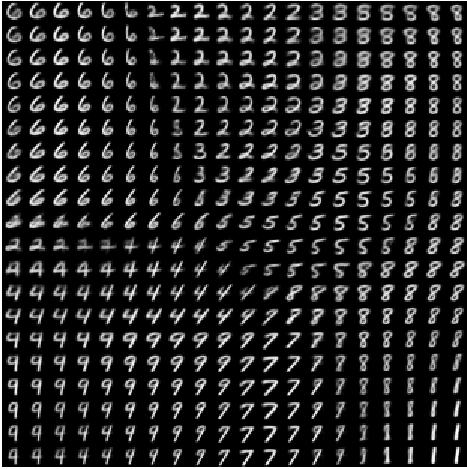
\includegraphics[height=7cm]{media/vae_manifold.pdf}
        \caption{Learned manifold using 2-dimensional latent space}
    \end{subfigure}%
    ~
    \begin{subfigure}[t]{0.5\textwidth}
        \centering
        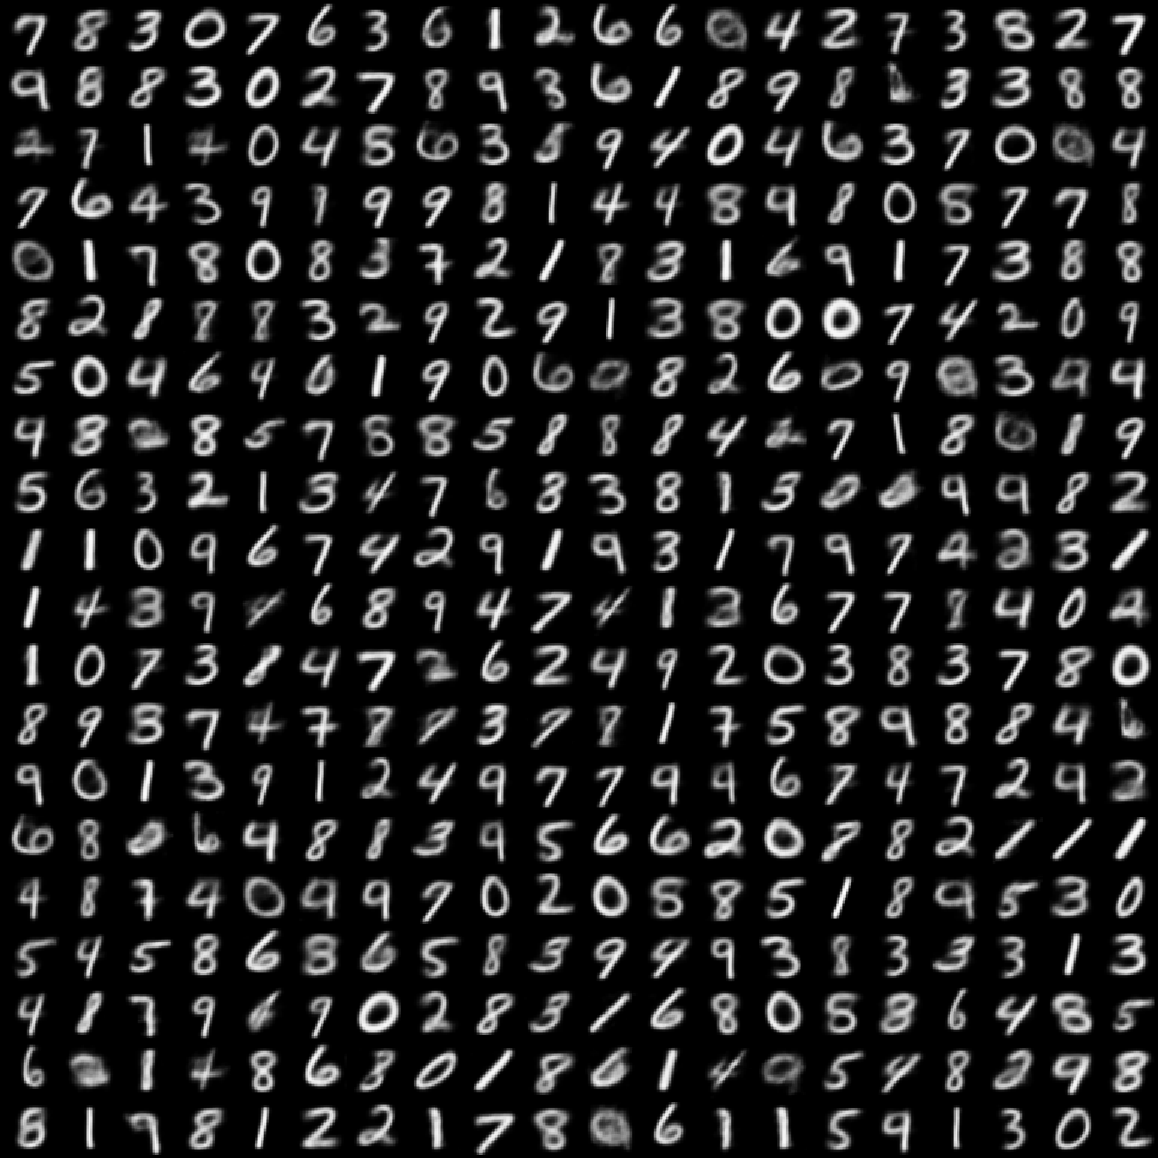
\includegraphics[height=7cm]{media/vae_samples.pdf}
        \caption{generated images by sampling from latent space and applying $p(x|z)$}
    \end{subfigure}
    \caption{Variational autoencoder learning performance}
\end{figure*}

%\subsection{Performance}
%\label{sub:vae_performance}

\newpage

\subsection{Extensions}
\label{sub:vae_extensions}

\subsubsection{Conditional VAE \cite{cvae:2015}}
\label{ssub:vae_conditional_vae}
Instead of using VAEs in a completely unsupervised manner on a unlabeled dataset, it is also possible to learn from datasets where a small subset of datapoints has corresponding labels while most datapoints are still unlabeled.
Techniques learning from such datasets are called semi-supervised learning and can improve performance significantly.\\

To adjust the VAE model to the semi-supervised case, we have to add an random variable $y$ corresponding to the corresponding label if available.
Thus we can extend the distributions as shown below.

%The modified setup of the semi-supervised case for the variational autoencoder can be formalized as follows.
%Dataset $X$ of size $N$ with observations $x_i$ with $i<N$ where for some small subset of observations $x_i$ the corresponding labels $y_i$ are known.
%We denote the labelled subset as $~p_l(x,y)$ and the unlabelled dataset as $~p_u(x,y)$.
%\begin{equation}

%\end{equation}
%Instead of randomly generated data, generation of output conditioned on some prior information is needed.
%A few examples would be super-resolution of images (citation!), prediction of subsequent frames of an video or other prediction tasks

%Conditional VAE is a modification of the original VAE framework to support conditioning on another variable $y$ in addition to the input data $x$.

%To support conditional distributions, the following relations have to be rewritten:
\begin{itemize}
\item \textbf{Sampling from data space}: $x \sim p_\theta(x|y,z)$ instead of $x \sim p_\theta(x|z)$.\\
\item \textbf{Probabilistic encoder}: $q_\theta(z|x,y)$ instead of just $q_\theta(z|x)$.\\
\item \textbf{Probabilistic decoder}: $p_\phi(x|y,z)$ instead of just $p_\phi(x|z)$.\\
\end{itemize}

These modifications allows us to formalize the new objective functionas shown in equations \ref{eq:cvae_labels} and \ref{eq:cvae_unknown}.

For datapoints $x$ where labels $y$ are available.
\begin{align}
  \label{eq:cvae_labels}
  \log p_\theta(x) &\geq \mathbb{E}_{q_\phi(z|x,y)} \bigg[\log p_\theta(x|y,z) + \log p_\theta(y) + \log p(z) - \log q_\phi(z|x,y)\bigg]
\end{align}

And for the unsupervised case where the label $y$ corresponds to an unknown entity, we treat $y$ as an additional latent variable.
\begin{align}
  \label{eq:cvae_unknown}
  \log p_\theta(x) &\geq \mathbb{E}_{q_\phi(y,z|x)} \bigg[\log p_\theta(x|y,z) + \log p_\theta(y) + \log p(z) - \log q_\phi(y,z|x)\bigg]
\end{align}

The final objective function for whole dataset is the summation between right-hand terms of equations \ref{eq:cvae_labels} for the labelled subset and \ref{eq:cvae_unknown} for the unlabelled subset.


\newpage

\subsubsection{Importance Weighted Autoencoder \cite{iwae:2015}}
\label{ssub:vae_importance_weighted_autoencoder}
% write about multiple stochastic layers

% write about k passes (just averages)

% write about IWAE, extends these k passes with importance weights
Importance Weighted Autoencoders (IWAE) extends on the VAE framework using $k$-sample importance weighting of the log-likelihood.
% add intuition for IWAE, ruslan explained it very well during his DL summer school talk! (talk_Montreal_2016_Salakhutdinov.pdf)
Using importance weighting can be informally interpreted as putting more weight on data with high likelihood.

The authors of the papers argue that using more samples will only tighten the lower variational bound.
$$
\log p(x) \geq \mathcal{L}_{k+1}(x) \geq \mathcal{L}_{k}(x)
$$

Additionally, if $\frac{p(h,x)}{q(h|x)}$ is bounded, then the model is guaranteed to reach the optimimum:
$$
\lim_{k \rightarrow \infty} \mathcal{L}_{k}(x) = \log p(x)
$$

Of course, using more samples will result in higher computational cost.

%\vspace{5cm}


\subsubsection{Deep Recurrent Attention Writer \cite{draw:2015}}
\label{ssub:vae_deep_recurrent_attention_writer}
The \emph{deep recurrent attention writer}\cite{draw:2015}, in short DRAW is an advanced extension of the variational autoencoder.
It uses recurrent neural networks as encoder as well as decoder and includes a selective attention mechanism.
These advancements allow the model to observe an image through a series of \emph{glimpses} and draw to an output region determined by the attention mechanism.
Without going into much detail, this allows the model to sequentially draw images in a way which resembles much of human-like drawing or sketching.


%It includes recurrent neural networks and a selective attention mechanism to 

%uses the selective attention mechanism in addition to a VAE with both recurrent encoder and recurrent decoder.
%DRAW allows to basically the pixels of an image sequentially very human-like.


\newpage
